% ====================================================================
%  RQ4 -- Applications beyond mortality (Chapter 6, ~5 min)
%  Layout convention: text/maths left, figure right.
% ====================================================================

\roadmapframe{4}{RQ4. How can survival prediction methods be applied to censored time-to-event outcomes beyond mortality, specifically time to fall in home care clients and time to degradation in ball bearings?}

\begin{frame}{Fall risk: time to a personal alarm}
\begin{columns}[c]
  \begin{column}{0.44\textwidth}
    \small
    \begin{itemize}
      \item Home care records from a Danish municipality (2021): \emph{what} care and \emph{how much}
      \item Event: personal alarm subscription within 26 weeks -- a proxy for falls; $\delta_i = 0$ otherwise
      \item 2,542 observations, 1,499 citizens, 49 covariates
      \item \textbf{95\% censored} (126 events)
    \end{itemize}
    \vspace{0.3em}
    Best: CoxBoost, C-index 0.64 (95\% CI 0.57--0.72). SHAP \cite{lundberg_unified_2017} on RSF \cite{ishwaran_random_2008}.
  \end{column}
  \begin{column}{0.54\textwidth}
    \centering
    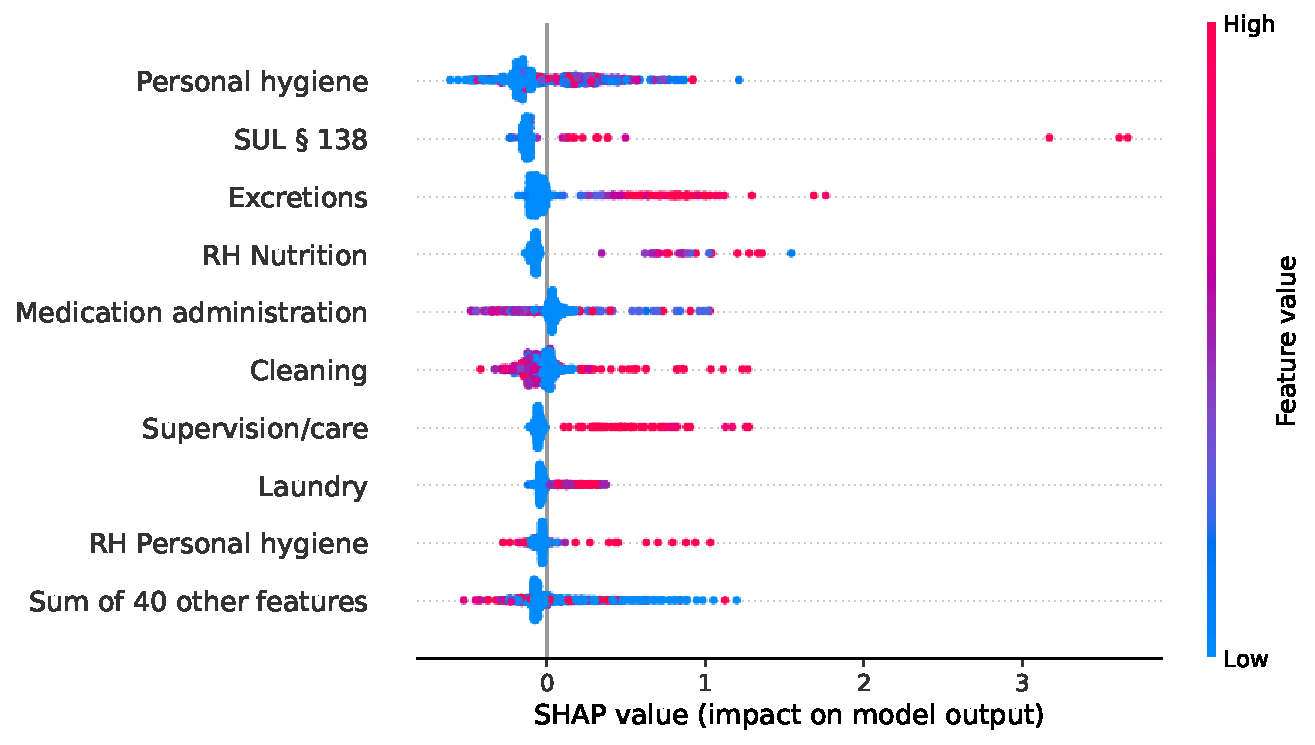
\includegraphics[width=\linewidth]{fall_shap_summary_plot.pdf}
    \figsource{Figure from Lillelund et al.~\cite{lillelund_prognosis_2026}}
  \end{column}
\end{columns}
\takeaway{Modestly better than chance at ranking who falls first (C-index 0.64) -- but with only 126 events, the time to fall (i.e., alarm subscription) could not be predicted reliably.}
\end{frame}

\begin{frame}{Bearings: define the event, then predict}
\begin{columns}[c]
  \begin{column}{0.44\textwidth}
    \small
    XJTU \cite{wang_hybrid_2020} and PRONOSTIA \cite{nectoux_pronostia_2012}: bearings run to failure under high load.
    \vspace{0.3em}
    \begin{itemize}
      \item \textbf{Event:} first time the vibration spectrum (FFT bins) deviates from normal operation -- well before failure
      \item \textbf{Covariates:} 12 time-domain features from two accelerometers, e.g.
      \[
        \text{RMS} = \Big(\tfrac{1}{N}\textstyle\sum_{i=1}^{N} x_i^2\Big)^{1/2}
      \]
      \item Censoring simulated (20\%)
    \end{itemize}
  \end{column}
  \begin{column}{0.54\textwidth}
    \centering
    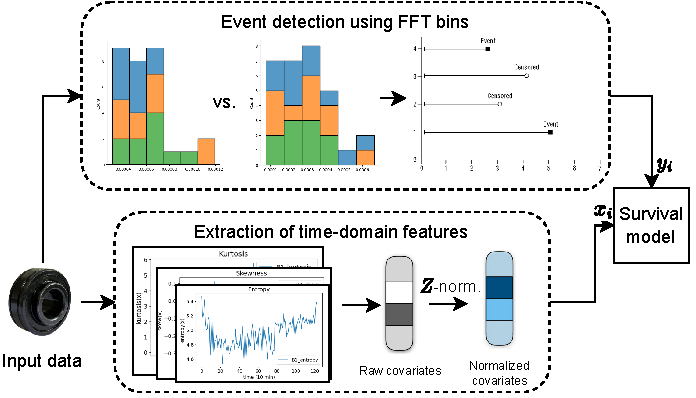
\includegraphics[width=0.7\linewidth]{bearing_pipeline.pdf}\\[0.2em]
    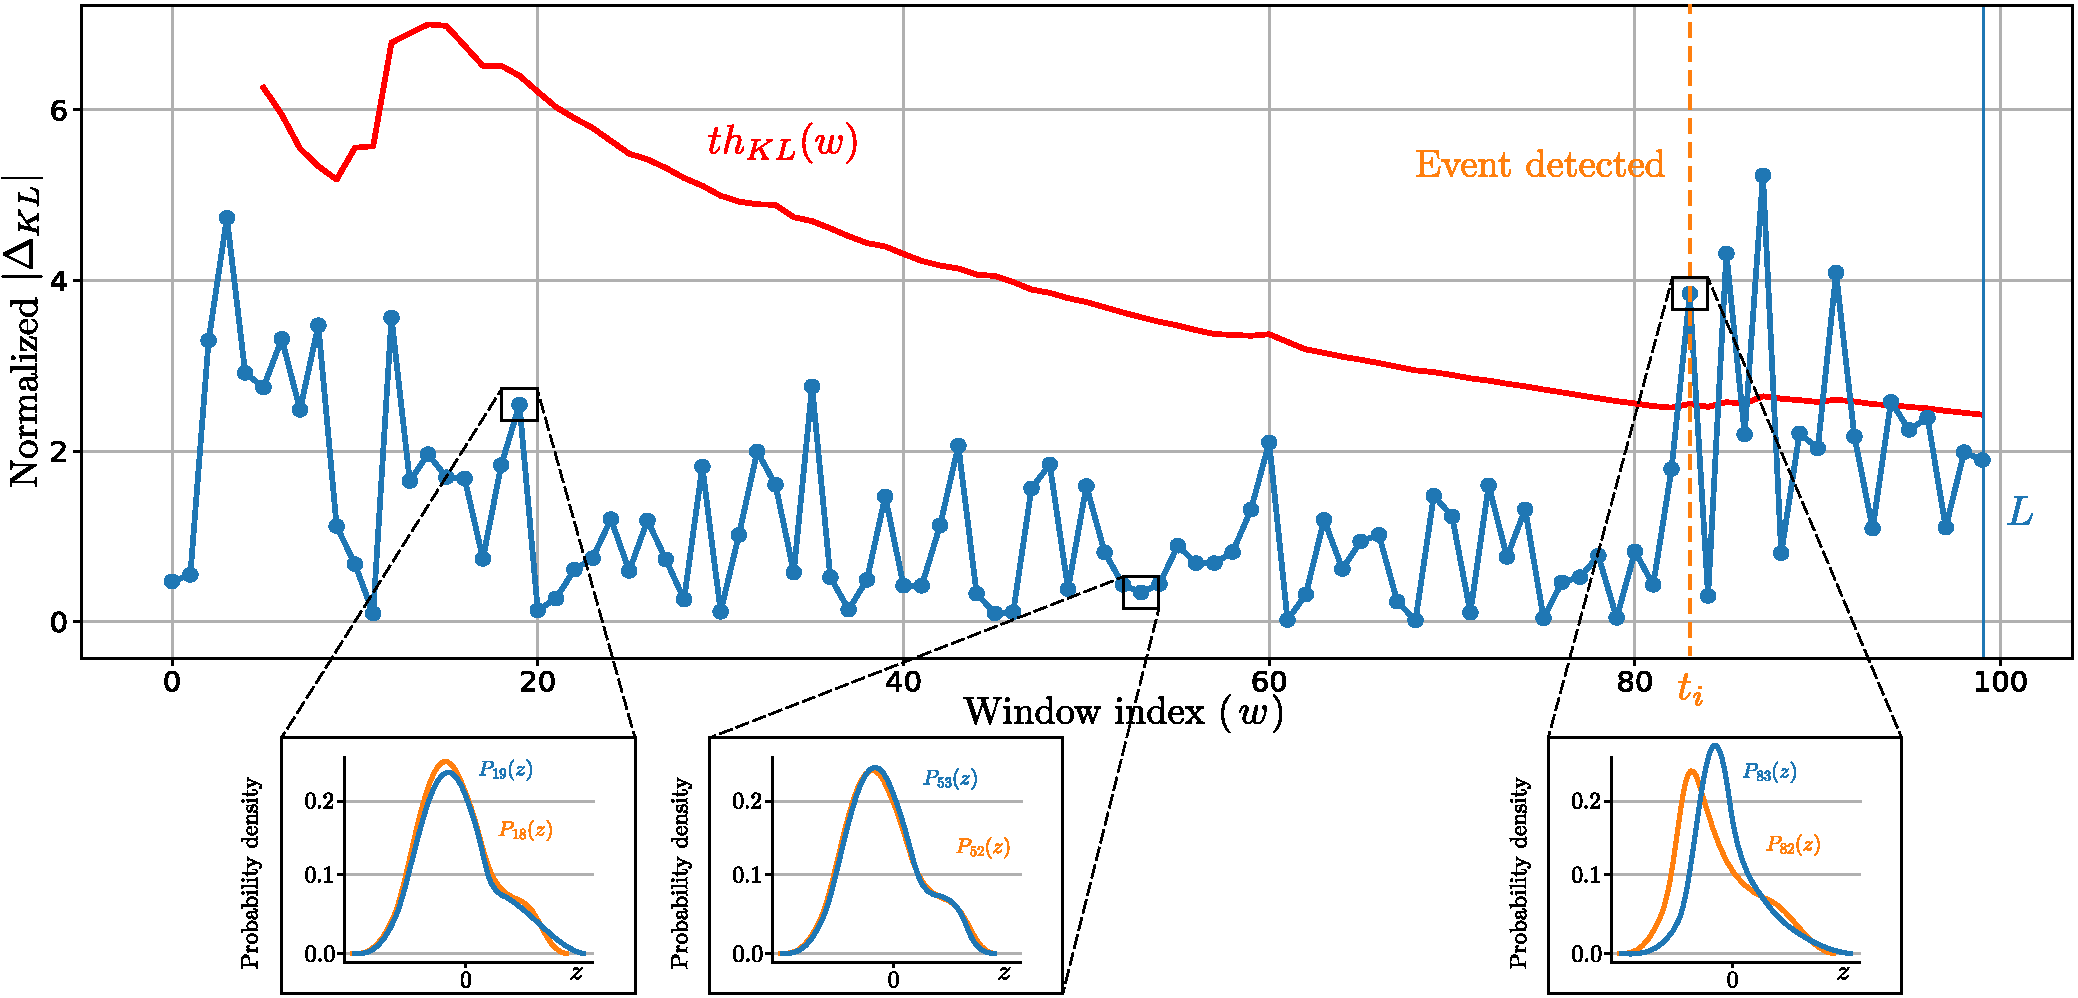
\includegraphics[width=\linewidth]{event_detector.pdf}
    \figsource{Figures from Lillelund et al.~\cite{lillelund_predicting_2023}}
  \end{column}
\end{columns}
\end{frame}

\begin{frame}{Higher vibration, earlier degradation}
\small Six survival models on XJTU; bearings split by RMS vibration ($\le 2$ vs.\ $> 2$).
\vspace{0.3em}

\begin{columns}[T]
  \begin{column}{0.32\textwidth}
    \centering
    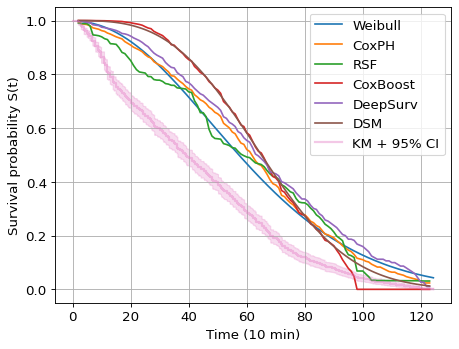
\includegraphics[width=\linewidth]{bearing_mean_survs.png}\\
    \scriptsize Mean predicted survival per model vs.\ KM
  \end{column}
  \begin{column}{0.32\textwidth}
    \centering
    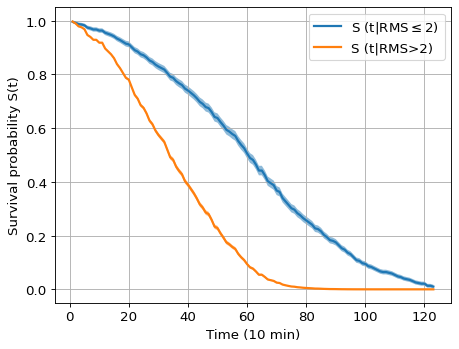
\includegraphics[width=\linewidth]{bearing_coxph_grouping.png}\\
    \scriptsize CoxPH: low vs.\ high RMS
  \end{column}
  \begin{column}{0.32\textwidth}
    \centering
    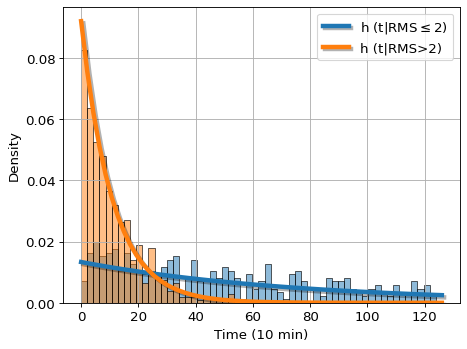
\includegraphics[width=\linewidth]{bearing_tte.png}\\
    \scriptsize Simulated times and hazards per RMS group
  \end{column}
\end{columns}
\figsource{Figures from Lillelund et al.~\cite{lillelund_predicting_2023}}
\takeaway{\footnotesize C-index up to 0.70 (XJTU) and 0.76 (PRONOSTIA) -- but from very few physical bearings.}
\end{frame}
